\scanpage{171}\mspage{26}
ceci de supposer que $X$ est ``localement homotopiquement trivial'', ce qui assure que le pro-ensemble simplicial que lui associent Artin-Mazur (par le procédé de nerfs de 'hyperrecouvrements) est essentiellement constant dans la catégorie homotopique ordinaire - donc $X$ définit un type d'homotopie habituel. Ce n'est \uline{pas} le cas bien sur pour le topos étale d'un schéma. Pour un tel cas, le $n$-groupoïde fondamental doit être conçu comme un \uuline{pro}-$n$-groupoïde (rien d'étonnant à cela, vu la théorie familière \unsure{du|des} $\pi_1$) ; et $\unsure{\mathcal E|E}_n$ comme une $(\mathrm{ind})$-$n$-catégorie (\unsure{le|la} ind-structure correspondant à l'exigence de locale trivialité, pour un $n$-champ variable, relativement à des recouvrements de plus en plus fins de $X$).

\figure{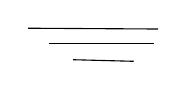
\begin{tikzpicture}[x=1cm,y=1cm]
\draw (0,0)--(1.65,-.01);
\draw (.27,-.19)--(1.60,-.19);
\draw (.57,-.40)--(1.34,-.42);
\end{tikzpicture}}

Je comprends cependant ta résistance instinctive à concevoir ce dépouillement extrême d'un beau topos $X$, au point de%
% Isolated short pen stroke at the right edge, between manuscript baselines 21 and 22; no textual interpretation.
\margin{\figure{\begin{tikzpicture}[x=1cm,y=1cm]\draw[line width=.5pt] (0,0)--(.14,.025);\end{tikzpicture}}}
n'en retenir que le maigre type d'homotopie. Bien plus, je suis persuadé qu'en%
% Isolated small black point at the lower right, below and right of the final n; origin uncertain, not assigned sentence punctuation.
\margin{\figure{\begin{tikzpicture}[x=1cm,y=1cm]\fill (0,0) circle[radius=.018];\end{tikzpicture}}}
% archive sheet number: 171
